\begin{apendicesenv}

\partapendices

\chapter{Modelo de Barema em Planilha do COLCIC}
\label{ap:modelo-barema-planilha}

Este apêndice apresenta o modelo de barema em planilha utilizado como referência no fluxo manual de preenchimento das Atividades Complementares. A planilha organiza as categorias de atividades, os limites de carga horária e os campos destinados ao preenchimento pelo discente, servindo também como base para o mapeamento das atividades e restrições posteriormente parametrizadas nos arquivos CSV da aplicação.

\begin{figure}[H]
    \centering
    \caption{Modelo de barema em planilha utilizado como referência para o preenchimento manual.}
    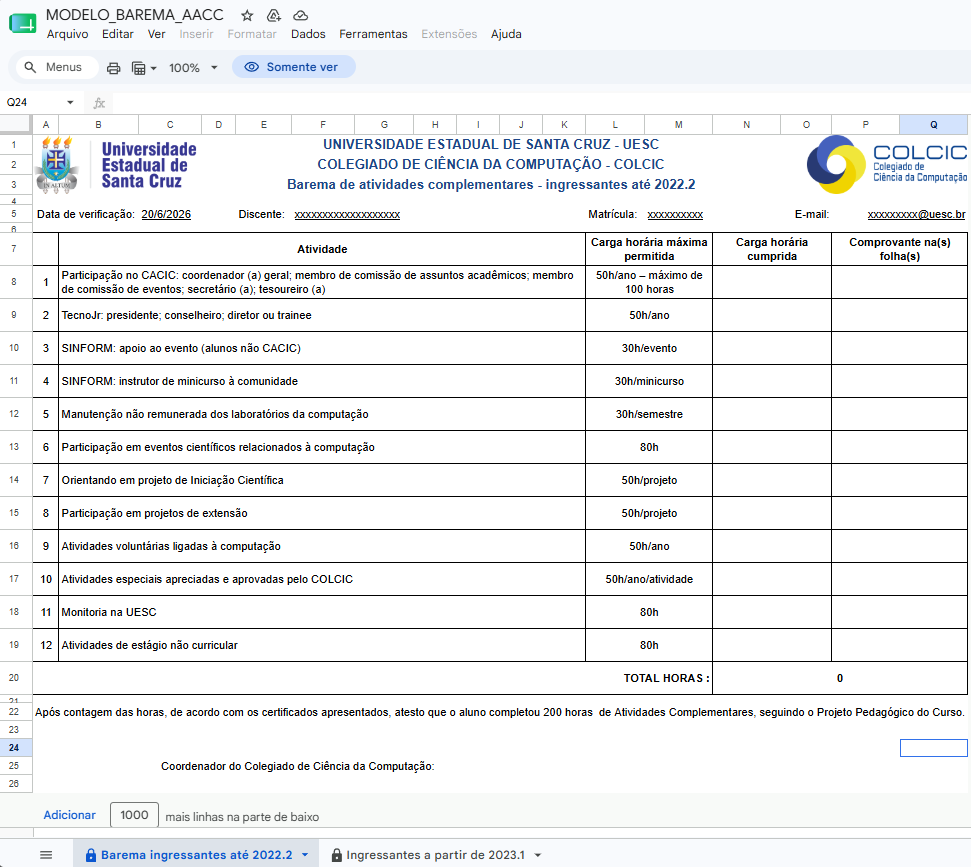
\includegraphics[width=\textwidth]{figuras/apendices/modelo_barema_planilha_colcic.png}
    \label{fig:modelo-barema-planilha-colcic}
    \legend{Fonte: Captura da planilha de barema do COLCIC (2026).}
\end{figure}

\end{apendicesenv}
